







\section{Multics and Unix at Bell Labs}

There is no avoiding Multics and UNIX if we are to discuss the development of compilers at Bell Labs.
We will cover the history of the American Telephone and Telegraph Company (AT\&T)
in \textit{very} broad strokes to contextualize the development of the programming languages
and compiler tools developed in this time period.

In very broad strokes, American Telephone and Telegraph Company (AT\&T) was a government-sanctioned
monopoly that provided telephone service to the United States.
They became a monopoly by buying up smaller telephone companies across the country.
Over time, they found they needed quite a bit of fundamental science in order to keep up with the
requirements of servicing the entire country, so in 1925 they created Bell Telephone
Laboratories in New York. If they did not continue providing quality service, the government could
(and very often did) threaten to break up the company, so this need was existential.

During the second world war, they expanded to New Jersey, early 1960s they moved to Murray Hill,
in suburban New Jersey, where they had a few thousand employees.
The laboratory was responsible solely for research, and thousands of other employees
worked on applying the research and developing the process knowledge needed to bring the
research into the phone system.
This research led to numerous fundamental discoveries and inventions in physics,
materials science and many more domains; these discoveries include the transistor, lasers,
fiber-optics and solar cells, to name a small subset.
Patents were the laboratory's primary measure of success, and they produced many.
At its peak, AT\&T was the nation's largest private employer with over 1 million employees.
If you are interested in an account of Bell Labs in anything close to the proper detail,
I recommend \textit{The Idea Factory} by Jon Gertner; our focus if far too narrow to do
it justice here.

In the early 1960s, the labs spun off a new department, the Computing Sciences Research Center,
off of the mathematics group. This group had about 25 people tasked with software and computing
research, which included operating systems.
In 1961, Fernando Corbat\'{o} at MIT created a timesharing system called CTSS,
or the Compatible Time Sharing System, with relative success.
In 1965 MIT set out to make a successor system with all kinds of enhancements; they partnered with
Bell Labs and General Electric to create the operating system called \textit{Multics}.
The machine was developed at GE (Multics required a special machine), Multics was designed at MIT,
and Bell Labs was responsible for large parts of the software development,
which was primarily done in IBM's PL/I programming language.
Ken Thompson described it as "monstrously over-engineered" and "typical second-system syndrome"
\cite{kernighan_interviews_thompson_2019};
while they had a wonderful time-sharing system in CTSS, they got too ambitious with thier sophomore project.
Ultimately, this project ran long past deadlines and was slow to run and altogether not what
the labs was hoping for, so in 1969 they pulled out of the project.
Honeywell took over Bell Labs' share of the project.

This left a bad taste in their mouths, and Bell Labs leadership sought to avoid operating
systems work in the wake of this venture.
Some of the members of the Multics team had other ideas; they had gotten a taste for
operating systems work, and now they had not operating system to work \textit{on}.
These included Ken Thompson, Dennis Ritchie, and Doug McIlroy.

At the time, Ken Thompson was researching file systems on an outdated and underused
Digital Equipment Corporation (DEC) PDP-7 machine.
He originally just used it for writing video games, until finally getting around to
his research on file systems.
He developed disc scheduling algorithms to maximize throughput on the PDP-7's disc drive.
To adequately test the performance of his file system algorithms, he needed some test
programs to stress the file system.
At some point in this process, he realized he was not far off from an
operating system of his own\cite{kernighan_interviews_thompson_2019}:

\begin{quotation}
At some point, I realized with out knowing it up until that point, that I was 
three weeks from operating system, with three programs, one a week. I needed an 
editor to write code, I needed an assembler to turn the code into language I 
could run, and I needed a kernel overlay, call it an operating system.  
Luckily, right at that moment, my wife went on a three-week vacation to take my 
one-year-old to visit her parents in California. One week, one week, one week, 
and we had Unix.
\end{quotation}

Thompson's assembler was not a complete toolchain; there were no libraries, linkers, or loaders.
The entire assembly program had to be presented to the assembler all at once,
and the output was directly executable. Thus the \texttt{a.out} naming convention for
the default executable output of modern compilers was born (\textit{a}ssembly \textit{out}put).
Even after the system gained more toolchain components, the name remained.

Very early on, Thompson's system picked up very impressive users.
Two at a time, Dennis Ritchie, Doug McIlroy, Morris McMahon, and Brain Kernighan
all became users on Thompson's new system.
They sent a proposal to get a PDP-10, which was top-of-the-line at the time,
to port Unix to a more powerful machine.
This was rejected as soon as Labs leadership saw it was related to operating systems,
in spite of the fact that their request was well within budget.
Joe Ossanna (another colleague) came up with a proposal that
positioned their need for a PDP-10 as a research project to develop better typesetting
software for filing patent applications (notably missing any mention of operating
systems).
Ossanna developed the Nroff and Troff typesetting programs to fullfil their claimed
goal of helping the patent office.
The patent office loved their software, and they ended up buying the computing group
a PDP-11 sometime in the early 1970s.
Unix came up on the PDP-11 almost immediately.
Thus we have the basis for discussing the subsequent development of compilers
and programming languages at Bell Labs.

\section{Personal Histories}

The following sections will feature many of the same figures;
here we will introduce them so their interleaving stories may be told
uninterrupted in the following sections.

\todo{Oral history of at least Ken Thompson, Dennis Ritchie, Brian Kernighan, Doug McIlroy.}

\subsection{Ken Thompson}
\subsection{Dennis Ritchie}
\subsection{Doug McIlroy}
\subsection{Donald Knuth}
\subsection{Brian Kernighan}
\subsection{Alfred Aho}
\subsection{Jeffrey Ullman}

\section{The First Unix Compilers}

It would not be inaccurate to describe this era of compiler history
as as cambrian explosion of programming languages and compiler tools, and
there were several reasons for that.
\todo{compiler-compilers, add intro.}
\todo{Ken Thompson, QED editor, first use of regex.}

We must also discuss Doug McIlroy if we are to discuss the early compilers;
he is described by nearly everyone at Bell Labs (who writes books or gives talks)
as the most brilliant member of that team that no one has heard of
\cite{kernighan_interviews_thompson_2019}, describing him as
"the smartest one of all of us and the least remembered or written down of all of us."
While Doug was the department head of the Computing Sciences Research Center,
he would regularly stop into the offices of his employees and drop ideas and requests
to them. In one case, he mentioned to Ken how convenient it would be to have
a tool for searching text files for patterns.
Ken already had a rough version of such a tool in his home directory,
so the next day he showed Doug his program and thus was born \texttt{grep};
many such tools came to be like this.

On another similar occasion, Doug walked into Ken's office to discuss the TMG language
(standing for TransMoGrifier),
designed by Robert McClure\cite{mcclure_tmg_compiler_compiler_1965}, one of his friends at the lab.
McClure had gotten defensive about this language, and when he left the lab,
he claimed it was proprietary and nobody else could use it.
TMG was a top-down recursive-descent compiler-compiler for context-free grammars
and procedural elements similar to Yacc, a tool to help write compiler
front-ends.
See this example from Doug's TMG manual\cite{tmg_manual_mcilroy_1972}
and notice the similarities to modern parser generators and Backus-Naur Form:

\begin{quotation}
This simple program defines the translation of fully parenthesized infix 
expressions to Polish postfix for a stack machine.
\begin{lstlisting}[frame=single]
    expr: <(>/exp1 expr operator expr <)> = { 3 1 2 };
    exp1: ident = { < LOAD > 1 };
    operator:
    op0: <+>/op1 = { < ADD > };
    op1: <->/op2 = { < SUB > };
    op2: <*>/op3 = { < MPY > };
    op3: </>     = { < DIV > };
\end{lstlisting}
\end{quotation}

Ken recounts\cite{kernighan_interviews_thompson_2019}
the story of how Doug brought a full TMG compiler \textit{written in TMG,
on paper} to Ken's office. He then decided to feed the TMG program into his TMG compiler
\textit{by hand} to produce an assembly listing of the TMG program.
He then went over to Ken's keyboard and typed in the program that his TMG-TMG compiler
had produced, and with astonishingly few errors, they had a working TMG compiler on the PDP-7.

Ken's logical next step was to use this new TMG compiler to
write a \ftn{} compiler for the PDP-7 because
"no computer was complete without \ftn{}."
Now, the PDP-7 was only 8k of 18-bit words of memory and Ken's Unix system needed
about half of that just to run, leaving only 4k for user programs.
Once completed, the new \ftn{} compiler took far more memory than was available for
user programs, so he had to cut down the TMG program to get a program small enough to
fit on the machine but capable enough to facilitate a usable programming language.
Once he finally cut down his compiler to 4k, he called that programming language \textit{B}.
His ill-fated attempt at producing a \ftn{} compiler ended up being a very different language,
based more so on BCPL than on \ftn{}
\footnote{The origins are really unclear. Ken himself mentions \ftn{} as his only inspiration
for B in a live interview\cite{kernighan_interviews_thompson_2019},
however Dennis Ritchie describes it as a "language of his own" and
"BCPL squeezed into 8K bytes of memory and filtered through Thompson's brain"
\cite{development_of_c_language_ritchie_1996}.
He describes the name as either a contraction of BCPL or (less likely) a contraction
of Bon, a language Thompson developed for Multics.}.
BCPL had been designed by Martin Richards at MIT in the mid-1960s, and thus had found
its way onto MIT's CTSS system, which Bell Labs employees were familiar with.

\section{BCPL, B, and C}

All three languages differ syntactically, but are semantically very similar,
and operate at a similar level of abstraction.
The BCPL compiler was allowed to use more memory than Thompson had on the PDP-7,
so it allowed for more complicated expression-oriented language features.
Dennis Ritchie points out the following two examples as only being possible
in BCPL and not in B or C due to memory constraints
\cite{development_of_c_language_ritchie_1996}:

\begin{lstlisting}[language=c,frame=single]
let P1 be (*@\textbfit{procedure}@*)
and P2 be (*@\textbfit{procedure}@*)
and P3 be (*@\textbfit{procedure}@*)

E1 := valof ( (*@\textbfit{declarations}@*) ;
              (*@\textbfit{commands}@*) ;
              resultis E2 ) + 1
\end{lstlisting}

Because the entire program was held in memory, the BCPL compiler could make
procedure \textbfit{P3} available to expressions inside procedure \textbfit{P1},
but the B compiler was limited to a one-pass technique and could not provide such features.
On the other hand, some BCPL features were purposefully left out of B; for example,
to share data between separately compiled source files, BCPL programs had to use
a global buffer. To make a procedure or variable available to other source files,
the programmer had to manually associate the name with an offset into this buffer,
similar to the \texttt{COMMON} block in \ftn{} programs.
In more mature B compilers and later in C, the linker handles this automatically.

\begin{figure}[h]
    \centering
    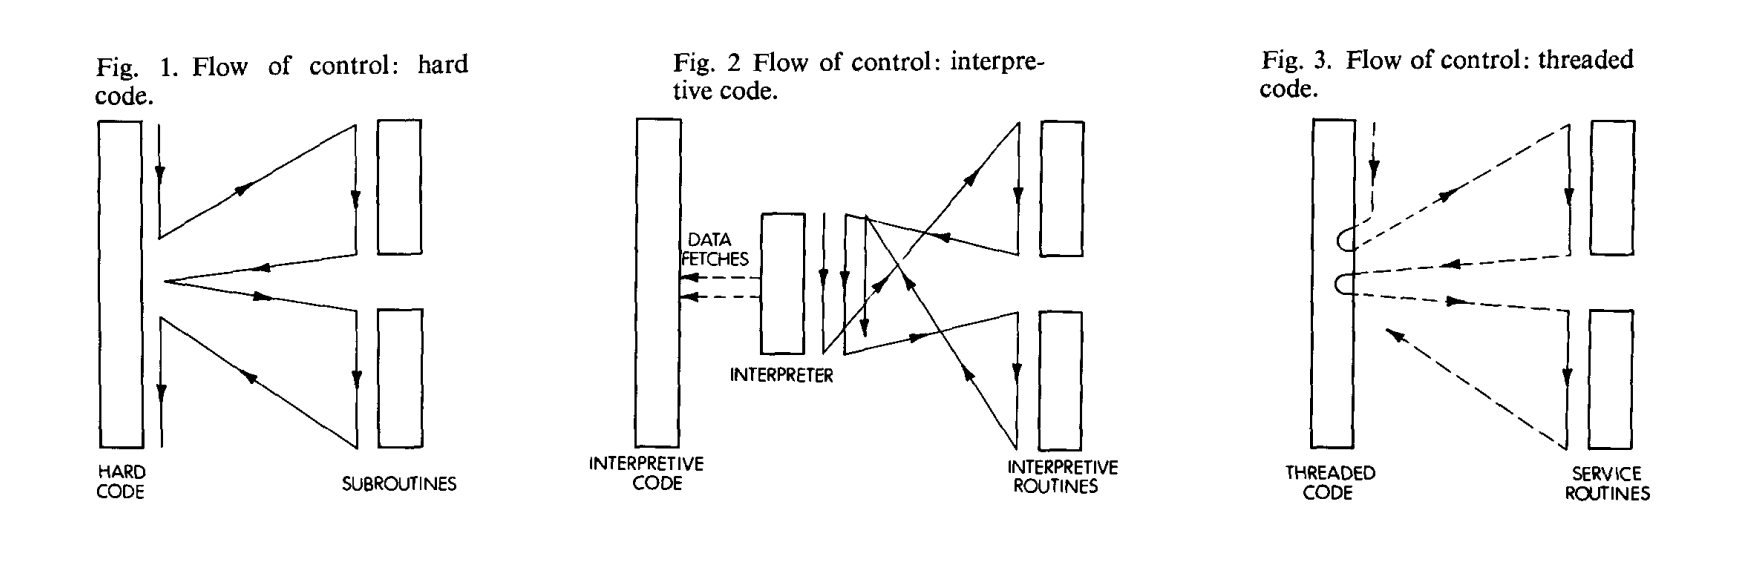
\includegraphics[width=0.8\textwidth]{resource/software/unix/bell-threaded-code-figures.png}
    \caption{Execution of Threaded Code\cite{bell_threaded_code_1973}}
    \label{fig:bell-threaded-code}
\end{figure}

The B compiler did not emit machine code directly, but instead used
\textit{threaded code}\cite{bell_threaded_code_1973}, an early form of \gls{bytecode},
which was then interpreted.
James Bell claimed that this threaded code needed no interpreter,
but really, the execution model for threaded code is just a specification
for an interpreter without outside the routines responsible for executing a given
bytecode instruction.
Today this would be considered a bytecode interpreter, but in the day when interpreters
were only known to interpret the source language directly, his ideas may have seemed
distinct from other forms of interpretation.
See Bell's depiction of the execution of threaded code \ref{fig:bell-threaded-code}.

Neither B nor BCPL had types; only the addressable size of data for the particular machine.
Since pointers were just integers representing offsets into memory, pointer arithmetic
was natural in both languages.

\section{Aho Before Bell Labs}

\section{Aho, Ullman, and Bell Labs}

\todo{Software (and compilers!) starts to become a real discipline!Ullman was older and further 
along than Aho, and Hopcraft came to Princeton and became Aho's advisor.}
\begin{quotation}
    One of the first people that I met at Princeton was a Columbia graduate by thename of Jeffrey 
Ullman. He had just gotten his undergraduate degree fromColumbia University and also had come to 
study digital systems in the EEdepartment at Princeton. So, he and I became close friends. When we 
graduated from Princeton, we both joined the newly formed Computing Sciences ResearchCenter at Bell 
Labs. There we developed a lifelong collaboration on subjects ranging from algorithms, programming 
languages, to the very foundations of computer science. I was very fortunate to have met some of the 
greatest people in the field and to have gotten to know them and work with them. You learn so much by 
working with the best people in the field. So, I felt very blessed because I had this kind of 
background
\dots
Hsu: Before we jump into Bell Labs more deeply, could you maybe explain-- talk about your PhD 
thesis,but try to explain it to somebody who, maybe like a museum goer who doesn't really know much 
about computer science and linguistics.

Aho: This is interesting. As I mentioned, Hopcroft told me, "Find your own research problem." He 
did teach a course in automata and language theory, so I got introduced to formal language theory 
and automata theory, at least, as it was known at that time. I was interested in programming 
languages and compilers. What I noticed was that a programming language has a syntax and a 
semantics. All languages have a syntax and a semantics. If you want to write a translator for a 
programming language, or even a natural language, you have to understand the syntax and semantics of 
your source language and the target language
\dots

Hansen: 1967, and you followed Ullman there. He had already joined Bell Labs before.

Aho: A few months before me.

Hansen: A few months before. And what group was it that you joined?

Aho: I was interviewed by a department head by the name of Doug McIlroy. He was an 
applied mathematician from MIT. He had been at Bell Labs for a few years before me. Amongst other 
things, he had co invented macros for programming languages and he's also in this class of one of the 
smartest people I've ever met.Jeff wanted to go to academia a little bit earlier than I did, like 
many years earlier. He stayed at Bell Labs for a few years and went to PrincetonUniversity where he 
joined the faculty of the electrical engineering department, but he would come and spend one day a 
week consulting at Bell Labs.His consulting stint was he would come Fridays and sit in my office 
all day.The conversations that we'd have would range over all sorts of topics, and sometimes he'd 
mentioned that he was working on a problem with a colleague atPrinceton, and after describing the 
problem, I might say, "You're kidding," and he said, "Oh, you're right. The solution is obvious, 
isn't it?" I don't know whether I would say dynamic programming or whatever, but several papers 
came out of this intense collaboration, and we got to the point where we could communicate with just 
a few words. We had a very large, shared symbol table.
\cite{aho_oral_history_2022}
\end{quotation}
\begin{quotation}
    But as Unix was being developed, Ken Thompson created the first two versions ofUnix using 
assembly language. He had joined Bell Labs at roughly the same time I had. He was there maybe six 
months or so ahead of us, and he had been assigned to work on the Multics project that BellLabs was 
part of with MIT and GE. When Bell Labs got tired of pouring money into Multics and not getting the 
operating system that it had wanted, it abandoned the project and left Ken Thompson to his 
own devices. Ken thought there were some good ideas in Multics. Being the genius that he was, he 
said, I can do it much more simply and much more elegantly. So he created a rudimentary version of 
Unix and thenkept writing and polishing it. Dennis Ritchie came on the scene. Ken had also created 
a programming language, B. The B was maybe the first letter of BCPL. Who knows? But when Dennis 
Ritchie looked at it, he said, what B needs is a decent type system. So he put a decent type system 
on B, and created theC programming language. Thompson and Ritchie wrote the third version of Unix 
using the newly createdC programming language. I became an early adopter of C, and I had C wired in 
my fingertips, so I could write C programs quite readily, and of course, there were all these neat 
tools that accompanied the programming environment on Unix. There were the text editors. I don't 
know whether you've ever heard of the ED editor or the QED editor that was at MIT as part of 
Multics. QED had regular expressions in it. This triggered my interest in regular expressions. Ken 
Thompson had written a program called grep for doing pattern matching on text files, and it had a 
very limited form of regular expressions when I encountered it.
\cite{aho_oral_history_2022}
\end{quotation}
\begin{quotation}
\textbf{Collaboration with Ullman}

Aho is best known for the textbooks he wrote with Ullman, his co-awardee. 
The two were full time colleagues for three years at Bell Labs, but after 
going back to Princeton as a faculty member Ullman continued to work one day a 
week for Bell.They retained an interest in the intersection of automata theory 
with formal language. In an early paper, Aho and Ullman showed how it was 
possible to makeKnuth's LR(k) parsing algorithm work with simple grammars that 
technically did not meet the requirements of an LR(k) grammar. This technique 
was vital to theUnix software tools developed by Aho and his colleagues at Bell 
Labs. That was just one of many contributions Aho and Ullman made to formal 
language theory and to the invention of efficient algorithms for lexical 
analysis, syntax analysis, code generation, and code optimization. They 
developed efficient algorithms for data-flow analysis that exploited the 
structure of "gotoless" programs, which were at the time just becoming the norm.
\cite{aho_turing_award_2020}
\end{quotation}
\begin{quotation}
\textbf{The Early History of Software, 1952-1968 101}

In the early 1960s computer science struggled to define itself and its 
purpose,in relation not only to established disciplines of electrical 
engineering and applied mathematics, but also in relation to—and as something 
distinct from—the use of computers on campus to do accounting, record keeping, 
and administrative work.58 Among those responsible for the discipline that 
emerged, Professor George Forsythe of Stanford's mathematics faculty was 
probably the most influential. With his prodding, a Division of Computer Science 
opened in the mathematics department in 1961; in 1965 Stanford established a 
separate department, one of the first in the country and still one of the 
most well-regarded.59
\cite{history_of_modern_computing_2003_ceruzzi}
\end{quotation}
\todo{Dragon book; all the books Aho, Ullman and others worked on together.}
\section{Compiler-Compilers}
\todo{Yacc and Lex made with Aho's help. then everyone started making mini languages.AWK. 
"Kernighan and Cherry developed a little language for specifyingmathematics called EQN using these 
tools"}
\begin{quotation}
    People started using the Kernighan and Lorinda Cherry EQN tool to specify mathematics in their 
documents and in the research papers that they were writing. They would feed the EQN specification 
into the typesetting program roff
\dots
Knuth adopted the EQN language to include in the TeX typesetting system, and in LaTeX. It's 
basically Kernighan and Cherry's way of specifying mathematics. These software tools had a great 
deal of influence, and Kernighan and Cherry enjoyed the fruits of parsing theory and formal language 
theory in using the tools Lex and Yacc to create their EQN typesetting language. Knuth has this 
saying that the best theory is motivated by practice and the best practice by theory. I internalized 
that with my early experience in the Computing SciencesResearch Center because I found that the 
theory that we were developing in computer science could be applied to document preparation systems, 
programming languages, compilers, and so on. It was really avery productive environment. I taught 
courses on compiler design at local universities, and then when I went to Columbia, I would teach 
the course on programming languages and their translators
\dots
I might point out that the first Fortran compiler developed by IBM in the 1950s took 18 staff years 
to create. In my programming languages and compilers course, I organized the students into teams of 
four or five. Each team had to create their own programming language, and then write a translator 
for it, and in all the time that I taught the course for almost 25 years at Columbia to thousands of 
students, never did a team failed to deliver a working compiler in the 15-week course, and I 
attribute that to the abstractions
\cite{aho_oral_history_2022}
\end{quotation}
\begin{quotation}
    Aho: Okay. AWK is a programming language that was created by me, Brian 
Kernighan, and Peter Weinberger.

Hsu: And it's your three initials that are in.

Aho: Yes. I'm the A in AWK. Weinberger is the W in AWK and Kernighan is the 
K in AWK.We thought that it was just a throwaway tool for us, nobody really 
would be interested in it. But it's amazing how much routine data processing 
there is in the world.The reason the language got to be known as AWK was because 
when our colleagues would see the three of us in one office or another, and when 
they'd walk past the open door, they'd say, AWK, AWK, AWK as they were going 
down the corridor. So we had no choice but to call it AWK because of the 
good-natured ribbing we got from our colleagues, and because at some Unix 
conference, they passed out t-shirts that had AWK,and the error message saying 
"bailing out on or near line five" on them.
\end{quotation}
\todo{Ratfor, AMPL, other Kernighan languages.}
\todo{continue with typesetting...}
\section{The Dragon Book}
\begin{quotation}
    Jeff had bought into this idea that it's good for your career to write a 
book about what you're working on. In the '70s, with all this work on Unix and 
C, there was a lot of interest in creating new programming languages and 
compilers. As with the algorithms book, what we did was we performed research 
on efficient algorithms for parsing and for some of the other phases of 
compilation, wrote papers on those  and presented them at conferences. But we 
took the important ideas that we developed and the community had developed over 
several decades and codified them into what are now called the dragon books. The 
first dragon book was published in 1977.We did have theorems and proofs in the 
book, and Jeff had this brilliant idea that the book should have a cover with a 
fierce dragon on it representing the complexity of compiler design,and then a 
knight in armor with a lance. The armor and the lance were emblazoned with 
techniques from formal language theory and compiler theory to slay the 
complexity of compiler design
\dots
In the 1980s, more was known about how to construct efficient compilers. We 
invited Ravi Sethi as a third coauthor, he was at Bell Labs at the time, to join 
us in creating the second version of the dragon book. In the first version, the 
dragon was in red. This second version, the dragon was-- sorry. In the first 
version it was in green. In the second version the dragon was in red. What was 
interesting about the red dragon book was there was a movie that was created in 
1995 titled Hackers with a young Angelina Jolie in it, and in the movie, there 
is the uber hacker that's explaining to the new hackers what you have to read to 
become an uber hacker. He shows them 10 papers and books that you must read, and 
one of them was the red dragon book. When my two children saw this movie, and 
they had seen the red dragon book at home, this is the first time they thought 
their old man was really something because he had one of his books in a 
Hollywood movie. It shows what you have to do to impress your kids these days. 
The red dragon book was 800 pages. In2007, we invited Monica Lam as a fourth 
coauthor to create a third version of the dragon book that had a purple dragon 
on the cover and it was close to a thousand pages. None of us had the heart to 
write a fourth book at this point because it just shows how much new knowledge 
had been created in the area of programming languages and compilers and their 
translators, and we continued to do research in this area to keep up with it.
\cite{aho_oral_history_2022}
\end{quotation}
\todo{Bjarne Stroustrup, C++ (1979); Dennis Ritchie, C (1972); Ken Thompson, B (1969); Brian 
Kernighan, AWK (1977), AMPL (1976), co-author of The C Programming Language (1978)}
